\documentclass[a4paper,12pt]{article}
\usepackage[ukrainian,english]{babel}
\usepackage{ucs}
\usepackage[utf8]{inputenc}
\usepackage[T2A]{fontenc}
\usepackage{amsmath}
\usepackage[document]{ragged2e}
\usepackage{graphicx}
\usepackage{wrapfig}
\usepackage[left=20mm, top=20mm, right=20mm, bottom=20mm, nohead, nofoot]{geometry}

\newcommand\tab[1][1cm]{\hspace*{#1}}
\newcommand\dint{\displaystyle\int}

\begin{document}
 \begin{justify}
 \thispagestyle{empty}\setlength{\parindent}{0pt}
  \topskip0pt
 \vspace*{\fill}
  \begin{center}
  \noindent\makebox[\linewidth]{\rule{\paperwidth}{0.4pt}}
   \LARGE{\bigbreak ДОМАШНЯ КОНТРОЛЬНА РОБОТА\\З ПРЕДМЕТУ\\''ДИФЕРЕНЦІАЛЬНІ РІВНЯННЯ''\\Варіант №15\bigbreak} 
   ФІ-12 Бекешева Анастасія 
   \noindent\makebox[\linewidth]{\rule{\paperwidth}{0.4pt}}
  \end{center}
 \vspace*{\fill}\newpage
 \begin{enumerate}
 	\item Знайти загальний інтеграл диференціального рівняння:
 		$$y'=\dfrac{x^2+2xy-y^2}{2x^2-2xy}$$
 		Запишемо у вигляді: $\dfrac{\partial y}{\partial x}=\dfrac{x^2+2xy-y^2}{2x^2-2xy}$. Зробимо заміну $y=xv$, тоді $\dfrac{\partial y}{\partial x}=x\dfrac{\partial v}{\partial x}+v$. Підставимо: $x\dfrac{\partial v}{\partial x}+v=\dfrac{x^2+2x^2v-(xv)^2}{2x^2-2x^2v};\tab x\dfrac{\partial v}{\partial x}+v=\dfrac{1+2v-v^2}{2-2v};\tab\dfrac1x\partial x=\\=\dfrac1{\left(\dfrac{1+2v-v^2}{2-2v}-v\right)}\partial v;\tab \dint\dfrac1x\partial x=\dint\dfrac{2-2v}{1+v^2}\partial v;\tab \ln|x|=\dint\dfrac{2\partial v}{1+v^2}-\\-\dint\dfrac{\partial (v^2+1)}{1+v^2}=2\arctan(v)-\ln|1+v^2|+C_1;\tab \ln|x|-2\arctan\left(\dfrac yx\right)-\ln\left|1+\dfrac{y^2}{x^2}\right|=C_1.$
 		$$\textbf{Відповідь: }\ln|x|-2\arctan\left(\dfrac yx\right)-\ln\left|1+\dfrac{y^2}{x^2}\right|=C_1.$$
 	\item Розв’язати задачу Коші:
 		$$y'+\dfrac2xy=x^3,\>y(1)=-\dfrac56$$
 		Вихідне рівняння є рівнянням Бернуллі. Стандартна заміна $y=uv$. Підставимо: $u'v+v'u+\dfrac2x uv=x^3;\tab \left(u'+\dfrac2xu\right)v+uv'=x^3$. Шукаємо частковий розв’язок рівняння: $u'+\dfrac2xu=0;\tab \dfrac{\partial u}u=-2\dfrac{\partial x}x;\tab \dint\dfrac{\partial u}u=-2\dint\dfrac{\partial x}x;\tab \ln|u|=\ln x^{-2}\\u=x^{-2}$. Підставимо: $x^{-2} v'=x^3;\tab \dint\partial v=\dint x^5\partial x;\tab v=\dfrac{x^6}6+C_1;\\y=x^{-2}\left(\dfrac{x^6}6+C_1\right)$. Врахуємо початкову умову: $-\dfrac56=1\left(\dfrac16+C_1\right);\tab C_1=-1.$
 		$$\textbf{Відповідь: } y=x^{-2}\left(\dfrac{x^6}6-1\right)$$
 	\item Розв’язати задачу Коші:
 		$$y'-y=2xy^2,y(0)=\dfrac12$$
 		Вихідне рівняння є рівнянням Бернуллі. Стандартна заміна $y=\dfrac1t, t'=-\dfrac{y'}{y^2}$. Поділемо рівняння на $y^2$: $\dfrac{y'}{y^2}-\dfrac1y=2x$. Підставимо: $t'+t=-2x$. Зробимо заміну $t=uv$. $u'v+v'u+uv=-2x;\tab (u'+u)v+v'u=-2x$. Шукаємо частковий розв’язок рівняння: $u'+u=0;\tab \dint\dfrac{\partial u}u=-\displaystyle\partial x;\tab u=e^{-x}$. Підставимо: $e^{-x}v'=-2x;\\\dint\partial v=-\dint2e^x\partial x;\tab v=-2e^x(x-1)+C_1;\tab t=-2(x-1)+C_1e^{-x};\\y=\dfrac1{-2(x-1)+C_1e^{-x}};\tab 0=\dfrac1{-2\left(\frac12-1\right)+C_1e^{-\frac12}};\tab C_1=0.$ 
 		$$\textbf{Відповідь: } y=\dfrac1{-2(x-1)}.$$
	\item Знайти рівняння лінії, що проходить через точку $M_0$, якщо відрізок її дотичної між точкою дотику та віссю $OY$ ділиться в точці перетину з віссю абсцис у відношенні $a:b$ (якщо рахувати від осі $OY$):
		$$M_0(1, -1),a:b=1:3$$
		\begin{figure*}[!h]
			\begin{center}
				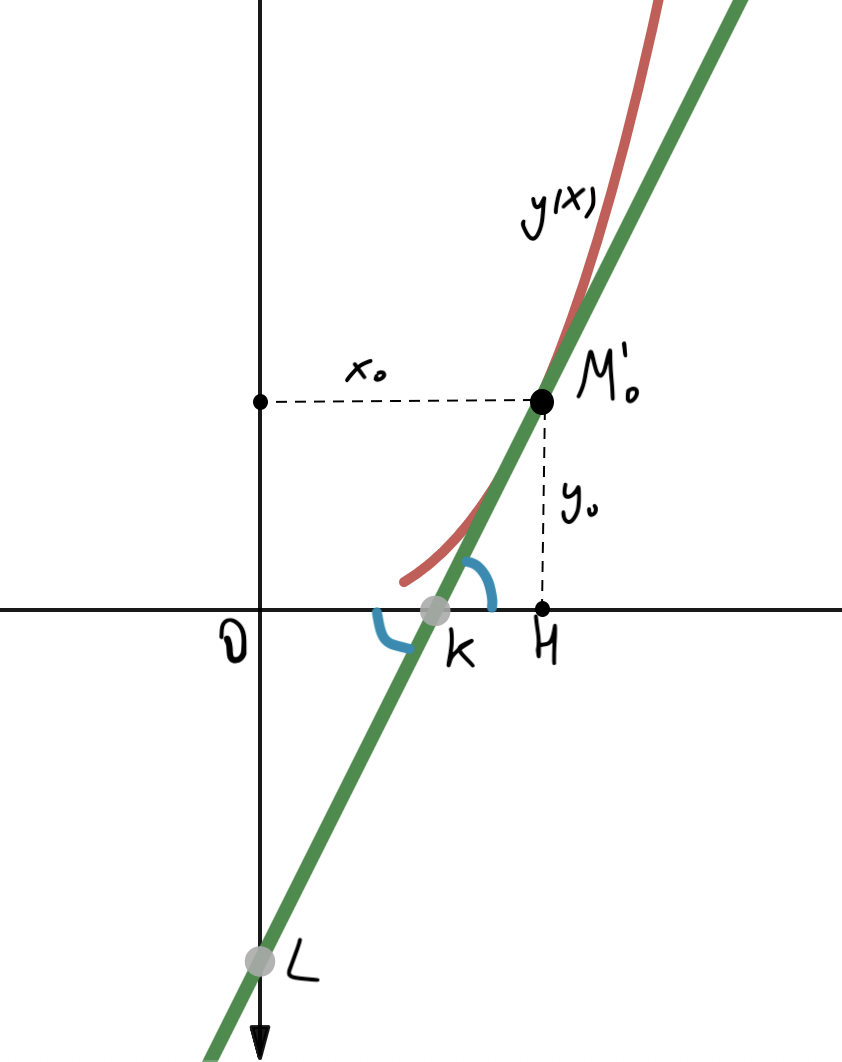
\includegraphics[scale=0.4]{plot_0.png}
			\end{center}
		\end{figure*}\\
		Розглянемо трикутники $OKL$ і $KM_0'H$, що подібні по двум кутам, тобто їх сторони пропорціональні: $\dfrac{|KL|}{|KM_0'|}=\dfrac{|OK|}{|KH|}=3$. Рівняння дотичної у точці $M_0'(x_0,y_0):y-y_0=\\=y'(x_0)(x-x_0)$. Щоб знайти де пряма пересікає вісь абсцис вирішемо c-му рівнянь: 
		$\begin{cases}
			y-y_0=y'(x_0)(x-x_0)\\y=0
		\end{cases};\tab -y_0=y'(x_0)(x-x_0);\tab xy'(x_0)=x_0y'(x_0)-y_0;\\x=x_0-\dfrac{y_0}{y'(x_0)}$. Таким чином: $K\left(x_0-\dfrac{y_0}{y'(x_0)},0\right)$. Знайдемо довільну точку $M(x,y)$ прямої (для зручності зробимо заміну $x_0=x, y_0=y$): $|OK|=\left|x-\dfrac{y}{y'}\right|;\\ |KH|=\left|x-\left(x-\dfrac{y}{y'}\right)\right|=\left|\dfrac{y}{y'}\right|;\tab |OK|=3|KH|;\tab \left|x-\dfrac{y}{y'}\right|=3\left|\dfrac{y}{y'}\right|;\\x-\dfrac{y}{y'}=\pm3\dfrac{y}{y'};\tab 
		\begin{cases}
			x=4\dfrac{y}{y'}\\x=-2\dfrac{y}{y'}
		\end{cases};\tab
		\begin{cases}
			\dint\dfrac{\partial y}{y}=4\dint\dfrac{\partial x}{x}\\\dint\dfrac{\partial y}{y}=-2\dint\dfrac{\partial x}{x}
		\end{cases};\tab
		\begin{cases}
			\ln|y|=\ln|C_1x^4|\\\ln|y|=\ln|C_2x^{-2}|
		\end{cases}$. Врахуємо точку $M_0(1,-1)$: $
		\begin{cases}
			-1=C_1^3\\-1=C_21^{-2}
		\end{cases};\tab C_1=C_2=-1;\tab y_1=-x^4,\\y_2=-x^2$. 
		$$\textbf{Відповідь: } y_1=-x^4, y_2=-x^2.$$
	\item Розв’язати задачу Коші:
		$$y''y^3+25=0,y(2)=-5, y'(2)=-1$$
		Вихідне рівняння має вид: $F(y, y', y'')=0$ і для зниження порядку покладемо $y'=p$. Тоді: $y''=pp';\tab pp'y^3=-25;\tab p\partial p=-25\dfrac{\partial y}{y^3};\tab p^2=25y^{-2}+C_1$. Врахуємо початкову умову: $1=25\cdot(-5)^{-2}+C_1;\tab C_1=0$. Тож: $y'=\dfrac{5}y$. Звідси: $y\partial y=5\partial x;\\\dint y\partial y=5\dint \partial x;\tab y^2=10x+C_2$. Врахуємо початкову умову: $25=10\cdot 2+C_2;\tab C_2=5$
		$$\textbf{Відповідь: } y^2-10x-5=0.$$
	\item Знайти загальний розв’язок диференціального рівняння: 
		$$y'''+4y''+4y'=(9x+15)e^x$$
		Складемо характеристичне рівняння: $\lambda^3+4\lambda^2+4\lambda=0;\tab \lambda(\lambda+2)^2=0;\\ \lambda_1=0,\lambda_2=-2$. Загальне рішення однорідного рівняння: $y_0=C_1+(C_2+C_3x)e^{-2}$.  Шукаємо частковий розв’язок $y_1=(Ax+B)e^x;\tab y_1'=(Ax+A+B)e^x;\\y_1''=(Ax+2A+B)e^x;\tab y_1'''=(Ax+3A+B)e^x$. Підставимо в початкове рівняння: $Ax+3A+B+4Ax+8A+4B+4Ax+4A+4B=9x+15;\tab 
		\begin{cases}
			9A=9\\15A+17B=15
		\end{cases};\\A=1, B=0$. Підставимо: $y_1=xe^x$. Загальне рішення: $y=y_1+y_0=xe^xC_1+\\+(C_2+C_3x)e^{-2}.$ 
		$$\textbf{Відповідь: } y=xe^xC_1+(C_2+C_3x)e^{-2}.$$
	\item Знайти загальний розв’язок диференціального рівняння: 
		$$y'''-16y'=48e^{4x}+64\cos4x-64\sin4x$$
		Складемо характеристичне рівняння: $\lambda^3-16\lambda=0;\tab\lambda_1=-4,\lambda_2=0,\\\lambda_3=4$. Загальне рішення однорідного рівняння: $y_0=C_1e^{-4x}+C_2+C_3e^{4x}$.  Шукаємо частковий розв’язок $y_1=Axe^{4x}+B\cos4x+C\sin4x;\tab y_1'=Ae^{4x}+4Axe^{4x}-4B\sin4x+4C\cos4x;\tab y_1''=8Ae^{4x}+16Axe^{4x}-16B\cos4x-16C\sin4x;\tab y_1'''=\\=48Ae^{4x}+64Axe^{4x}-64B\sin4x+64C\cos4x$. Підставимо в початкове рівняння: $48Ae^{4x}+64Axe^{4x}-64B\sin4x+64C\cos4x-16Ae^{4x}-64Axe^{4x}+64B\sin4x-64C\cos4x=\\=48e^{4x}+64\cos4x-64\sin4x;\tab-48e^{4x}+32Ae^{4x}-64\cos4x-128C\cos4x+64\sin4x+\\+128B\sin4x=0;\tab e^{4x}(32A-48)-\cos4x(128C+64)+\sin4x(128B+64)=0\\
		\begin{cases}
			32A-48=0\\128B+64=0\\128C+64=0
		\end{cases};\tab 
		\begin{cases}
			A=\dfrac32\\B=-\dfrac12\\C=-\dfrac12
		\end{cases}$. Підставимо: $y_1=\dfrac32xe^{4x}+-\dfrac12\cos4x+-\dfrac12\sin4x$. Загальне рішення: $y=y_1+y_0=\dfrac32xe^{4x}+-\dfrac12\cos4x+-\dfrac12\sin4x+C_1e^{-4x}+C_2+C_3e^{4x}$
		$$\textbf{Відповідь: } y=\dfrac32xe^{4x}+-\dfrac12\cos4x+-\dfrac12\sin4x+C_1e^{-4x}+C_2+C_3e^{4x}.$$		
	\item Розв’язати задачу Коші:
		$$y''+4y=4\cot2x,y\left(\dfrac\pi4\right)=3,y'\left(\dfrac\pi4\right)=2$$
		Складемо характеристичне рівняння: $\lambda^2+4=0;\tab\lambda_1=-2i,\lambda_2=2i$. Загальне рішення однорідного рівняння: $y_0=C_1\sin2x+C_2\cos2x$. Складемо матрицю Вронського: 
		$W=\begin{pmatrix}
			\sin2x &\cos2x\\2\cos2x&-2\sin2x
		\end{pmatrix};\tab W^{-1}=
		\begin{pmatrix}
			\sin2x&\dfrac{\cos2x}2\\\cos(2x)&-\dfrac{\sin2x}2
		\end{pmatrix};\\ \overline{C}'=
		\begin{pmatrix}
			\sin2x&\dfrac{\cos2x}2\\\cos(2x)&-\dfrac{\sin2x}2
		\end{pmatrix}
		\begin{pmatrix}
			0\\4\cot2x
		\end{pmatrix}=
		\begin{pmatrix}
			\dfrac{2\cos^22x}{\sin2x}\\-2\cos2x
		\end{pmatrix};\tab\overline{C}=\begin{pmatrix}
			\dint\dfrac{2\cos^22x}{\sin2x}\partial x\\\dint-2\cos2x\partial x
		\end{pmatrix}.\\ \dint\dfrac{2\cos^22x}{\sin2x}\partial x=\dint\dfrac{\cos^22x}{\sin2x}\partial(2x)=\dint\cos2x\cot2x\partial(2x)=-\dint\sin2x\partial(2x)+\\+\dint\dfrac1{\sin2x}\partial(2x)=\cos2x-\ln|\cot x|+C_1.\\\dint-2\cos2x\partial x=-\dint\cos2x\partial(2x)=-\sin2x+C_2.\\\overline{C}=
		\begin{pmatrix}
			\cos2x-\ln|\cot x|\\-\sin2x
		\end{pmatrix}+C$.  Шукаємо частковий розв’язок $y_1=-\cos2x\sin2x+\\+2\left(\dfrac12\cos2x-\dfrac12\ln|\cot x|\right)\sin2x=-\ln|\cot x|\cdot\sin2x$. Загальне рішення: $y=y_1+\\+y_0=C_1\sin2x+C_2\cos2x-\sin2x\ln|\cot x|$. Врахуємо початкову умову: $\\
		\begin{cases}
			3=C_1\sin\left(2\cdot\dfrac\pi4\right)+C_2\cos\left(2\cdot\dfrac\pi4\right)-\sin\left(2\cdot\dfrac\pi4\right)\ln\left|\cot \left(\dfrac\pi4\right)\right|\\
			2=-2\cos\left(2\cdot\dfrac\pi4\right)\ln|\cot \left(\dfrac\pi4\right)|+\dfrac{\sin\left(2\cdot\dfrac\pi4\right)}{\sin \left(\dfrac\pi4\right)\cos \left(\dfrac\pi4\right)}-2C_1\sin\left(2\cdot\dfrac\pi4\right)+2C_2\cos\left(2\cdot\dfrac\pi4\right)
		\end{cases}.\\C_1=0,C_2=3;\tab y=-\sin2x(\ln|\cot x|-3).$
	$$\textbf{Відповідь: } y=-\sin2x(\ln|\cot x|-3).$$
 	
 \end{enumerate}
 
 
 
 
 
 
 
 
 
 
 
 
 
 
 
 
 
 
 \end{justify}
\end{document}